\section{INTRODUCTION}

% It is a challenging testbed for robotics algorithms
Table tennis is a challenging game for humans to master. For robots it also serves as a testbed to study and validate the effectiveness of different movement generation algorithms. Combining different estimation, movement generation and execution schemes and studying how close they come to imitating expert human behaviour will yield important insights for robotics research.

Optimality plays an important role in the search for efficient and feasible striking trajectories. However, so far most of the robots used for table tennis were too specialized to require any nontrivial planning. Furthermore, most algorithms for robotic table tennis focused on simplifications of the game that fixed any additional degrees of freedom of the robot in order to quickly come up with a movement plan. In this paper, we show the advantages of incorporating optimality in trajectory generation to create more flexible movement, at the cost of some additional computation. 
% refs needed

Our robotic setup with an anthropomorphic seven degree of freedom Barrett WAM arm is shown in Figure~\ref{robot}. The redundant arm is custom made and capable of high speeds and accelerations. It is a good platform to study different movement generation schemes. Optimal control based approaches have the potential to make use of all degrees of freedom in planning, contributing to more natural and efficient generation of strikes. % ref needed

\begin{figure}[t!]
\center
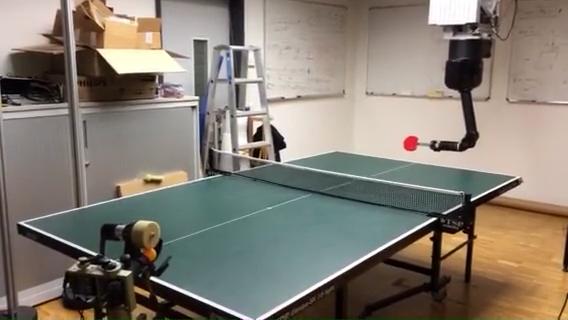
\includegraphics[scale=0.4]{robot1.png}			
\caption{Robotic table tennis setup with four cameras on the corners of the ceiling tracking the ball at 60 Hz. We filter the raw ball data provided from the cameras with an Extended Kalman Filter and predict the ball trajectory well in advance of the trajectory generation. A constrained nonlinear optimization problem is solved to find an optimal striking trajectory as well as an optimal striking time.}
\label{robot}
\end{figure}
% REPLACE PHOTO WITH ANOTHER ONE INCLUDING CAMERAS

Our contributions are two-fold. Firstly, we come up with an optimal control framework where the generation of striking trajectories are the result of an optimization problem. As opposed to previous works, we do not use any inverse kinematics or any fixed plane when computing joint trajectories. Secondly, we do not rely on the simplistic racket-ball reflection model when computing desired racket velocities and orientations. Instead, we train a probabilistic model based on human ball-racket demonstrations and use it to calculate cautious strategies for returning the ball.

In the rest of this paper, we describe the trajectory generation framework in detail. First we introduce previous work on table tennis and other relevant trajectory generation frameworks. In Section~\ref{method} we formalize robot trajectory generation as a specific optimal control problem and incorporate probabilistic modeling within this framework. In Section~\ref{alg} we discuss a two-stage optimization approach for optimizing the previously introduced cost functional. In Section~\ref{results} we evaluate the performance of this approach and compare it with previous inverse kinematics (IK) approaches. Experiments in our robotic table tennis setup are given. Finally, in the conclusions we discuss several promising extensions for this framework. %VHP-based

\begin{figure}[t!]
\centering
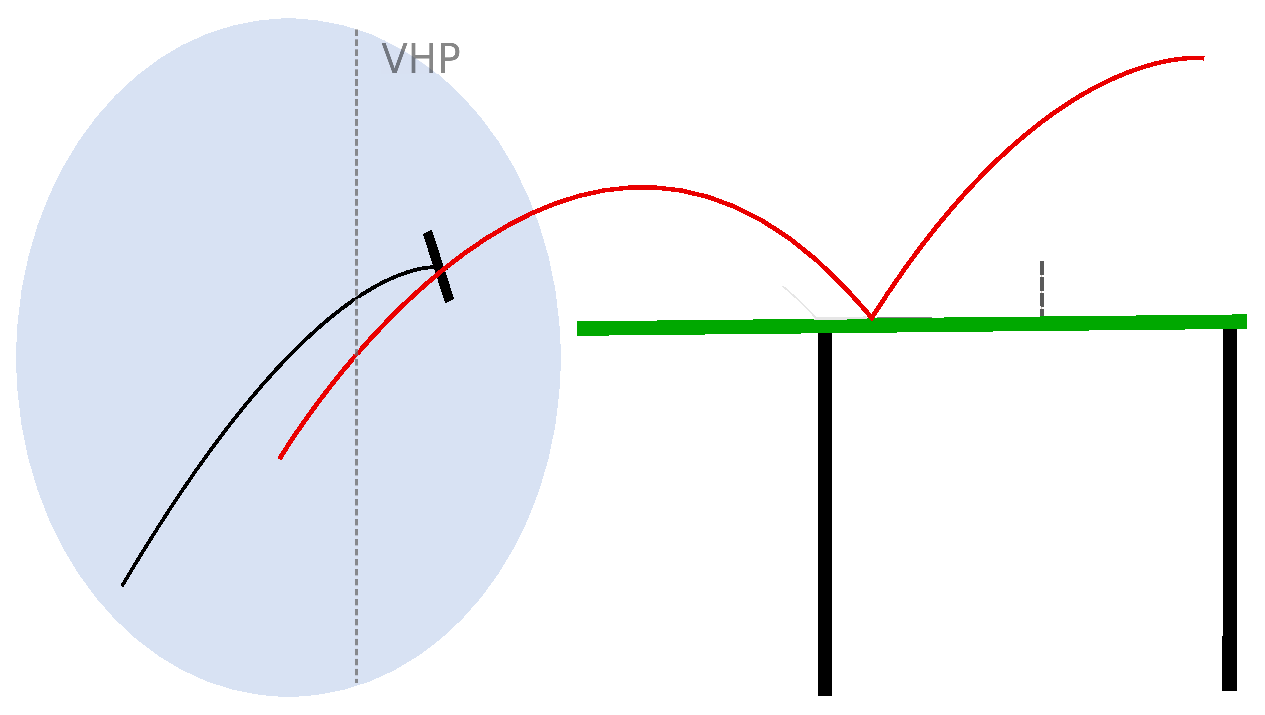
\includegraphics[scale=0.4]{drawing.eps}			
\caption{Illustrating the main idea behind this paper: fixing a virtual hitting plane (VHP) can make the generated trajectories unnecessarily restrictive and the resulting inverse kinematics may be infeasible. We instead consider the whole ball trajectory in our trajectory generation framework and optimize for the hitting time as well as the hitting point. Racket trajectory and the mean of the ball trajectory are shown in black and red, respectively. VHP is shown as a dotted gray line, the workspace of the robot is shown as an ellipsoidal light blue region.}
\label{mainIdea}
\end{figure}